% !TEX encoding = UTF-8
% !TEX TS-program = pdflatex
% !TEX root = ../tesi.tex
% !TEX spellcheck = it-IT

%**************************************************************
\chapter{Verifica e validazione}
\label{cap:verifica-validazione}
%**************************************************************

\section{Test di unità}
L'approccio Test Driven garantisce intrinsecamente che ogni unità software sia testata ancora prima della sua implementazione. Ogni unità dovrebbe contenere il quantitativo minimo di codice necessario a far rendere positivo il test ideato e scritto in precedenza.\\
Questo approccio, sebbene all'inizio sia piuttosto insolito ed a prima vista tedioso, risulta invece essere imprescindibile nello sviluppo di applicazioni web, soprattutto utilizzando framework JavaScript. AngularJS stesso è stato pensato per scrivere applicazioni facilmente testabili, includendo al suo interno delle librerie create appositamente per il testing.\\
Mi è stato quindi possibile testare ogni componente della logica dell'applicazione, controllando il comportamento delle unità e dei loro metodi. Tramite l'utilizzo di sistemi di automazione, nel mio caso \emph{Karma}, sono riuscito a rendere il processo di testing quanto più automatico possibile ed a calcolare con facilità le metriche base per verificare l'utilità dei test scritti.\\
Tramite il plugin di \emph{coverage} di Karma, ho generato automaticamente tali cifre, suddividendole per:
\begin{itemize}
	\item line coverage;
	\item statement coverage;
	\item branch coverage;
	\item function coverage.
\end{itemize}
Nella figura sottostante, presento i dati in forma tabellare, come vengono visualizzati dall'output del plugin \emph{karma-coverage}, installabile facilmente da \gls{npm}.

%DA CAMBIARE LA WIDTH, PERCHE' COSI' FA' CAGARE, PLZ. >_<
\begin{figure}[!h] 
    \centering 
    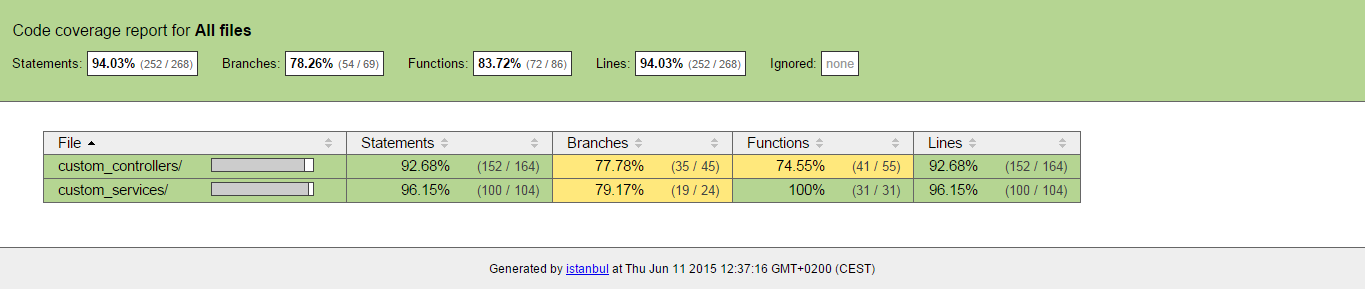
\includegraphics[width=\paperwidth]{coverage/coverage_all} 
    \caption{Metriche di copertura nel progetto SkillMatrix}
\end{figure}

%**************************************************************
\section{Test End-To-End}